\documentclass{beamer}
\usepackage[T2A]{fontenc}
\usepackage[utf8]{inputenc}
\usepackage[english, russian]{babel}
\usepackage{graphicx}
\graphicspath{{images/}}

\usetheme{Madrid}
\usecolortheme{beaver}

\title{Математическая модель импульсного погружателя с учетом малой асинхронности}
\date{25.06.2021}
\author{Бабошин Сергей Дмитриевич}

\setbeamertemplate{frametitle}[default][center]
\setbeamertemplate{navigation symbols}{}
\setbeamertemplate{footline}[page number]
\setbeamertemplate{caption}[numbered]

\begin{document}

    \frame{\titlepage}

    \begin{frame}
        \frametitle{Постановка задачи}
        В данной работе ставятся и решаются следующие задачи:
        \begin{enumerate}
            \item Описать математическую модель взаимодействия элементов системы: ипмульсного погружателя,
            сваи и грунта;
            \item Получить численное решение для уравнения, представляющего собой модель процесса погружения сваи;
            \item Сравнить полученные результаты с результатами, полученными в ходе практических испытаний.
        \end{enumerate}
    \end{frame}

    \begin{frame}
        \frametitle{Импульсный погружатель}
        \begin{figure}
            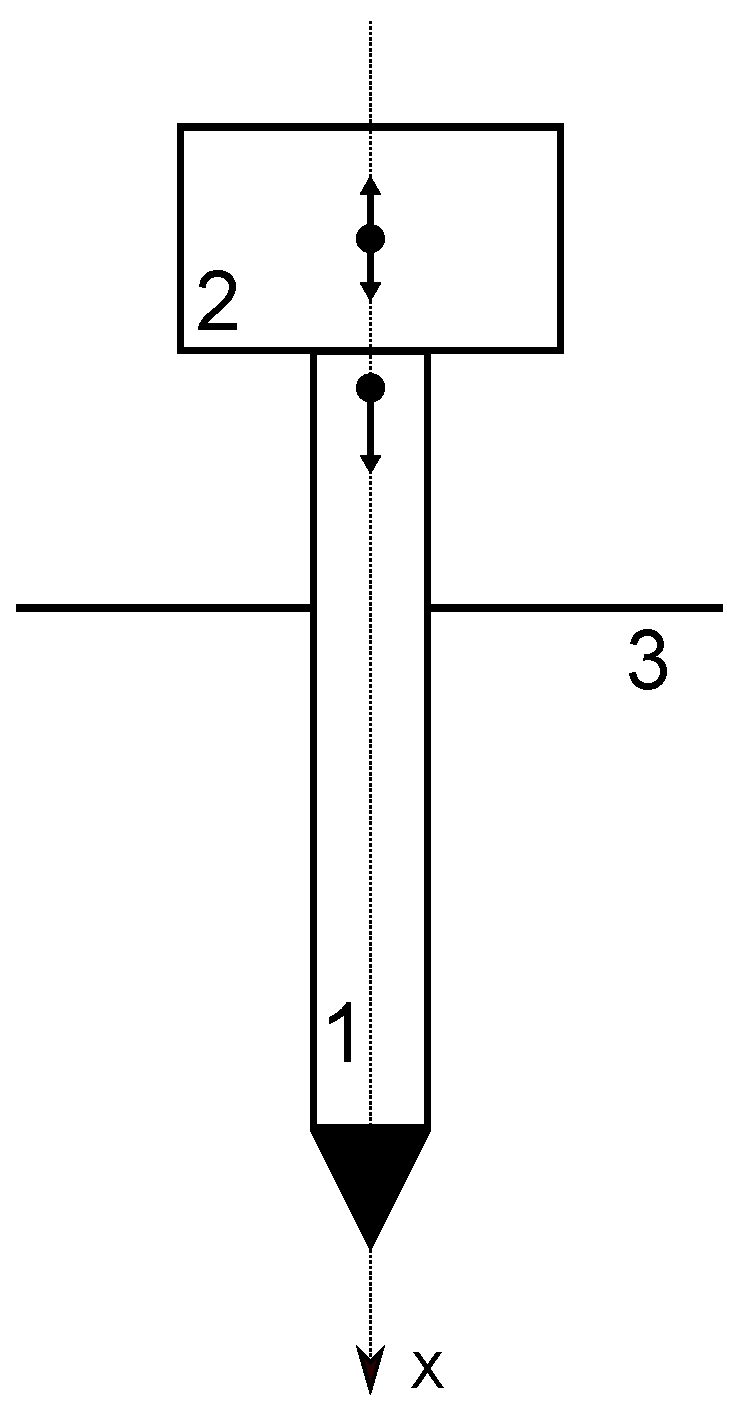
\includegraphics[width=0.2\linewidth]{pogruzhatel}
            \caption{Модель импульсного погружателя.}
        \end{figure}
        \begin{align*}
            1 &- \text{погружаемый элемент } (\textit{свая}),\\
            2 &- \textit{вибровозбудитель},\\
            3 &- \textit{грунт}.
        \end{align*}
    \end{frame}

    \begin{frame}
        \frametitle{Процесс погружения сваи}
        Процесс вибрационного погружения можно описать с помощью следующего равенства:
        \begin{equation}
            \label{eq:R}
            R = F_\text{вибр. возд.} + F_\text{тяж.} - F_\text{бс} - F_\text{лс},
        \end{equation}
        где
        \begin{equation*}
            \begin{aligned}
                &R - \text{равнодействующая сила,}\\
                &F_\text{вибр. возд.} - \text{сила, создаваемая погружающей установкой,}\\
                &F_\text{тяж.} - \text{сила тяжести,}\\
                &F_\text{бс} - \text{сила бокового сопротивления,}\\
                &F_\text{лс} - \text{сила лобового сопротивления.}
            \end{aligned}
        \end{equation*}
    \end{frame}

    \begin{frame}
        \frametitle{Численное моделирование}
        \begin{itemize}
            \item $R = ma = m\ddot{x}$, {\scriptsizeгде $m$ - масса и $a$ - ускорение.}
            \item $F_\text{тяж.} = mg$, {\scriptsizeгде $g$ - ускорение свободного падения.}
            \item $F_\text{лс} = S_\text{пс} h_i(x(t), \xi)$, {\scriptsizeгде $S_\text{пс}$ - площадь поперечного сечения
            сваи, $h_i(x(t), \xi)$ - удельное лобовое сопротивление, $\xi$ - коэфициент условий работы грунта под нижним
            концом сваи.}
            \item $F_\text{бс} = P x(t) f_i(\psi)$, {\scriptsizeгде $P$ - периметр сваи, $x(t)$ - глубина погружения и $f_i(\psi)$ - удельная
            сила бокового сопротивления, зависящая от типа грунта.}
            \end{itemize}
        Переписав уравнение \ref{eq:R} получаем следующее дифферециальное уравнение второго порядка:
        \begin{equation}
            \label{eq:main}
            m\ddot{x} = F_\text{вибр. возд.} + mg + S_\text{пс} h_i(x(t), \xi) + P x(t) f_i(\psi)
        \end{equation}
        с начальными условиями:
        \begin{equation*}
            x(0) = 0, \dot{x}(0) = 0.
        \end{equation*}
    \end{frame}

    \begin{frame}
        \frametitle{Численное решение}
        Рассмотрим разностную аппроксимацию дифференциального оператора $L_{xx} = \ddot{x}$ на равномерной сетке с шагом $h$:
        \begin{equation}
            \label{eq:lxx}
            L_{xx} = \ddot{x} = \frac{x(t + h) - 2x(t) + x(t - h)}{h^2}
        \end{equation}
        Заменив $\ddot{x}$ в уравнении \ref{eq:main} разностной аппроксимацией \ref{eq:lxx}, получаем:
        \begin{equation*}
                x_{i+1} = 2x_i - x_{i-1} + \frac{h^2}{m}(F_\text{вибр. возд.} + mg + S_\text{пс} h_i(x(t), \xi) + P x(t) f_i(\psi)),
        \end{equation*}
        где $x_i = x(t_i)$ и 
        \begin{equation*}
            x_0 = 0, x_1 = 0
        \end{equation*}
        Данное рекурентное равенство лежит в основе расчёта глубины погружения.
    \end{frame}

    \begin{frame}
        \frametitle{Программа для расчёта процесса погружения}
        \begin{figure}
            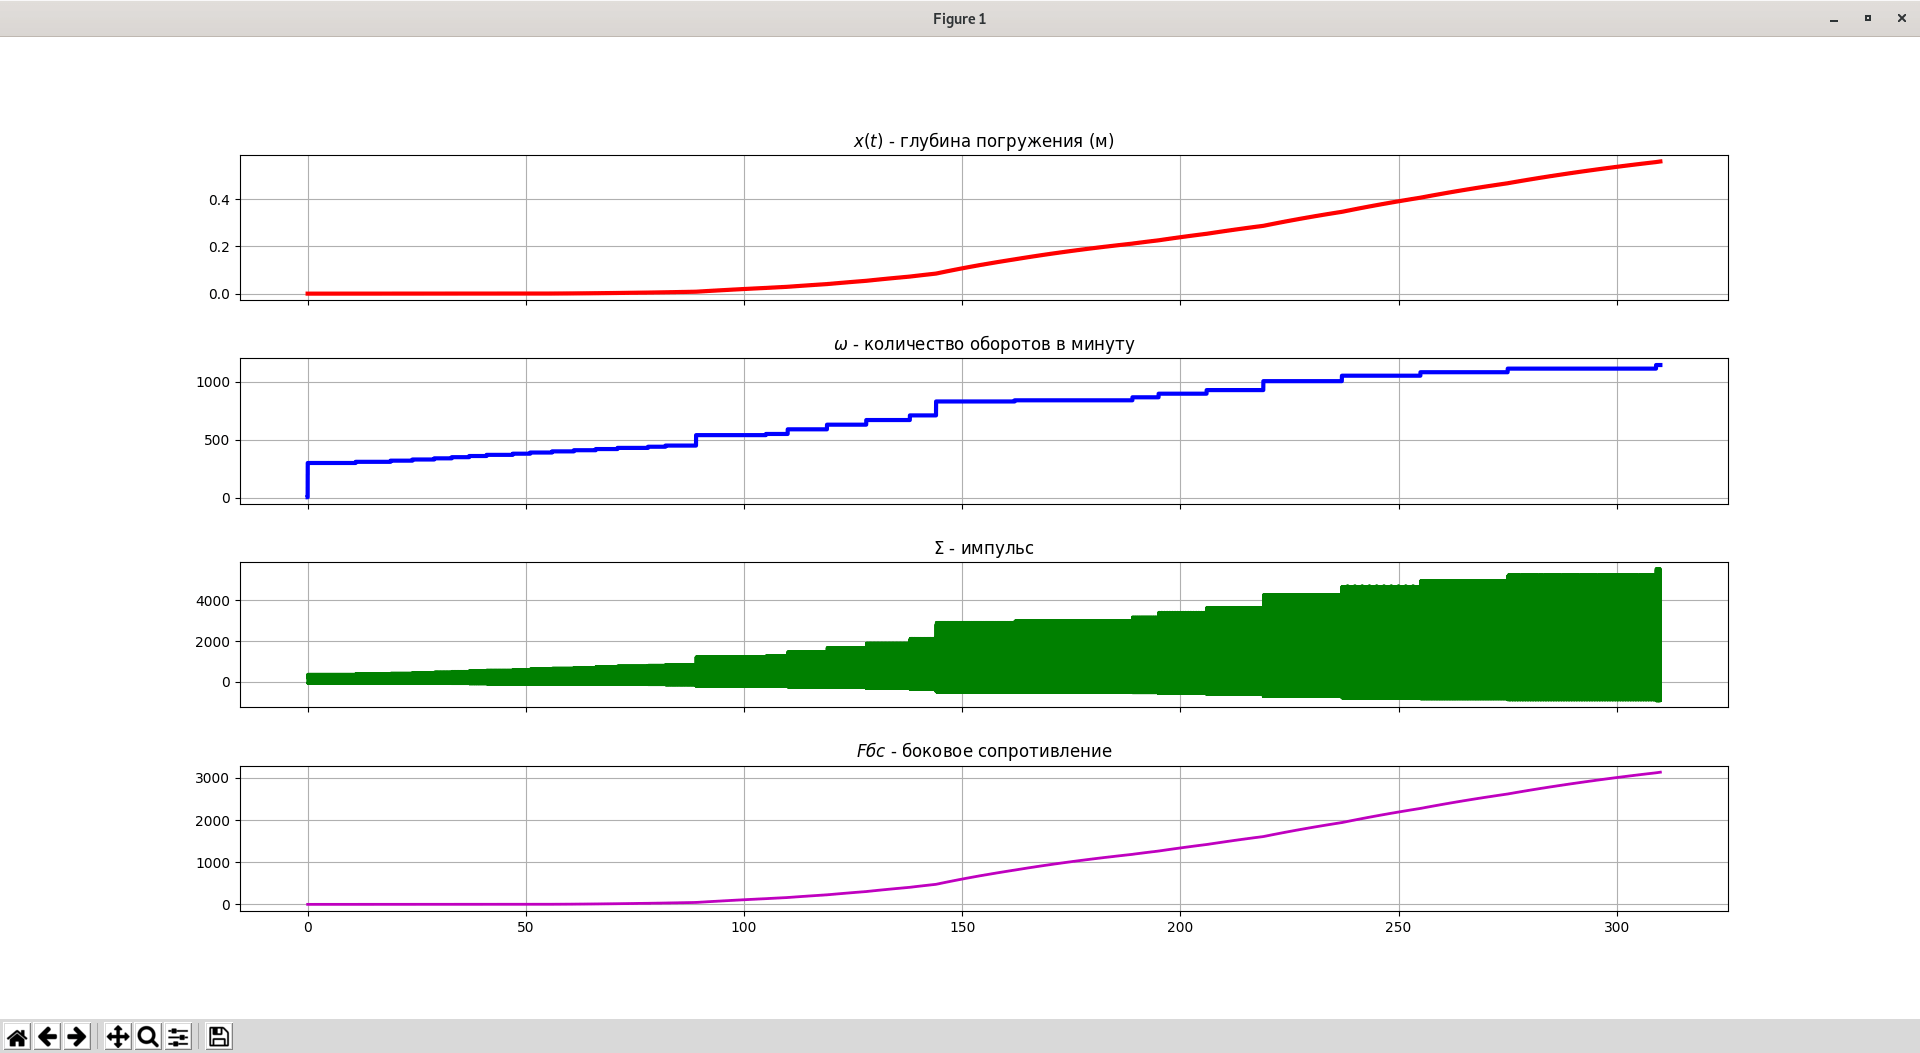
\includegraphics[width=0.7\linewidth]{screenshot}
            \caption{Скриншот окна программы.}
        \end{figure}
        \begin{columns}
 
            \column{0.3\textwidth}
            \begin{figure}
                
\includegraphics[width=0.8\linewidth]{python-logo}
            \end{figure}
             
            \column{0.3\textwidth}
            \begin{figure}
                
\includegraphics[width=0.8\linewidth]{matplotlib-logo}
            \end{figure}

            \column{0.3\textwidth}
            \begin{figure}
                
\includegraphics[width=0.8\linewidth]{numpy-logo}
            \end{figure}

            \end{columns}
    \end{frame}

    \begin{frame}
        \frametitle{Программа для расчёта процесса погружения}
        \begin{figure}
            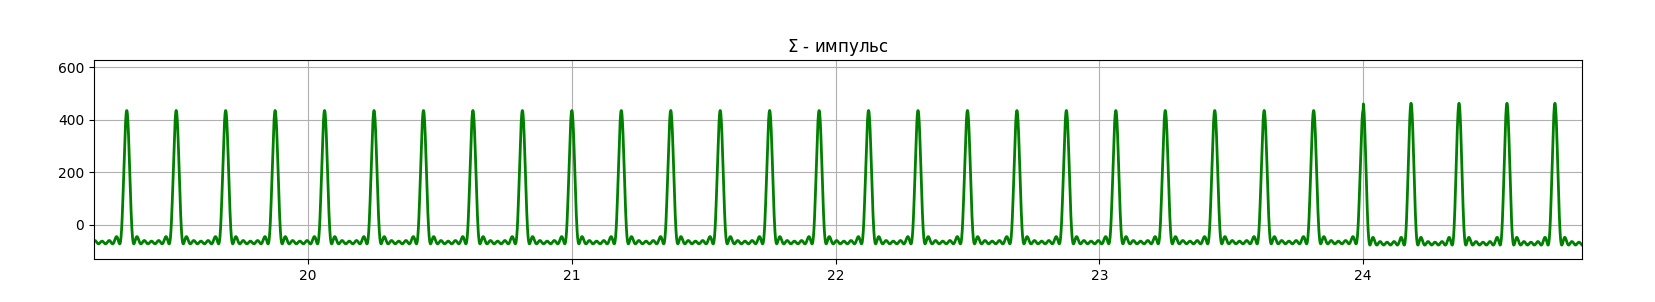
\includegraphics[width=1\linewidth]{graph-impulse}
            \caption{График силы, генерируемой импульсным погружателем.}
        \end{figure}
    \end{frame}

    \begin{frame}
        \frametitle{Условия практических испытаний}
        Для проверки результатов, использовалась свая со следующими параметрами:
        \begin{itemize}
            \item Свая представляет собой квадратную трубу с размером 40x40 мм и толщиной стенки 2 мм,
            \item Длина сваи - 1,7 м,
            \item Масса сваи - 4,17 кг.
        \end{itemize}
        Масса испульсного погружателя - 37 кг.
    \end{frame}

    \begin{frame}
        \frametitle{Результаты работы пограммы}
        \begin{figure}
            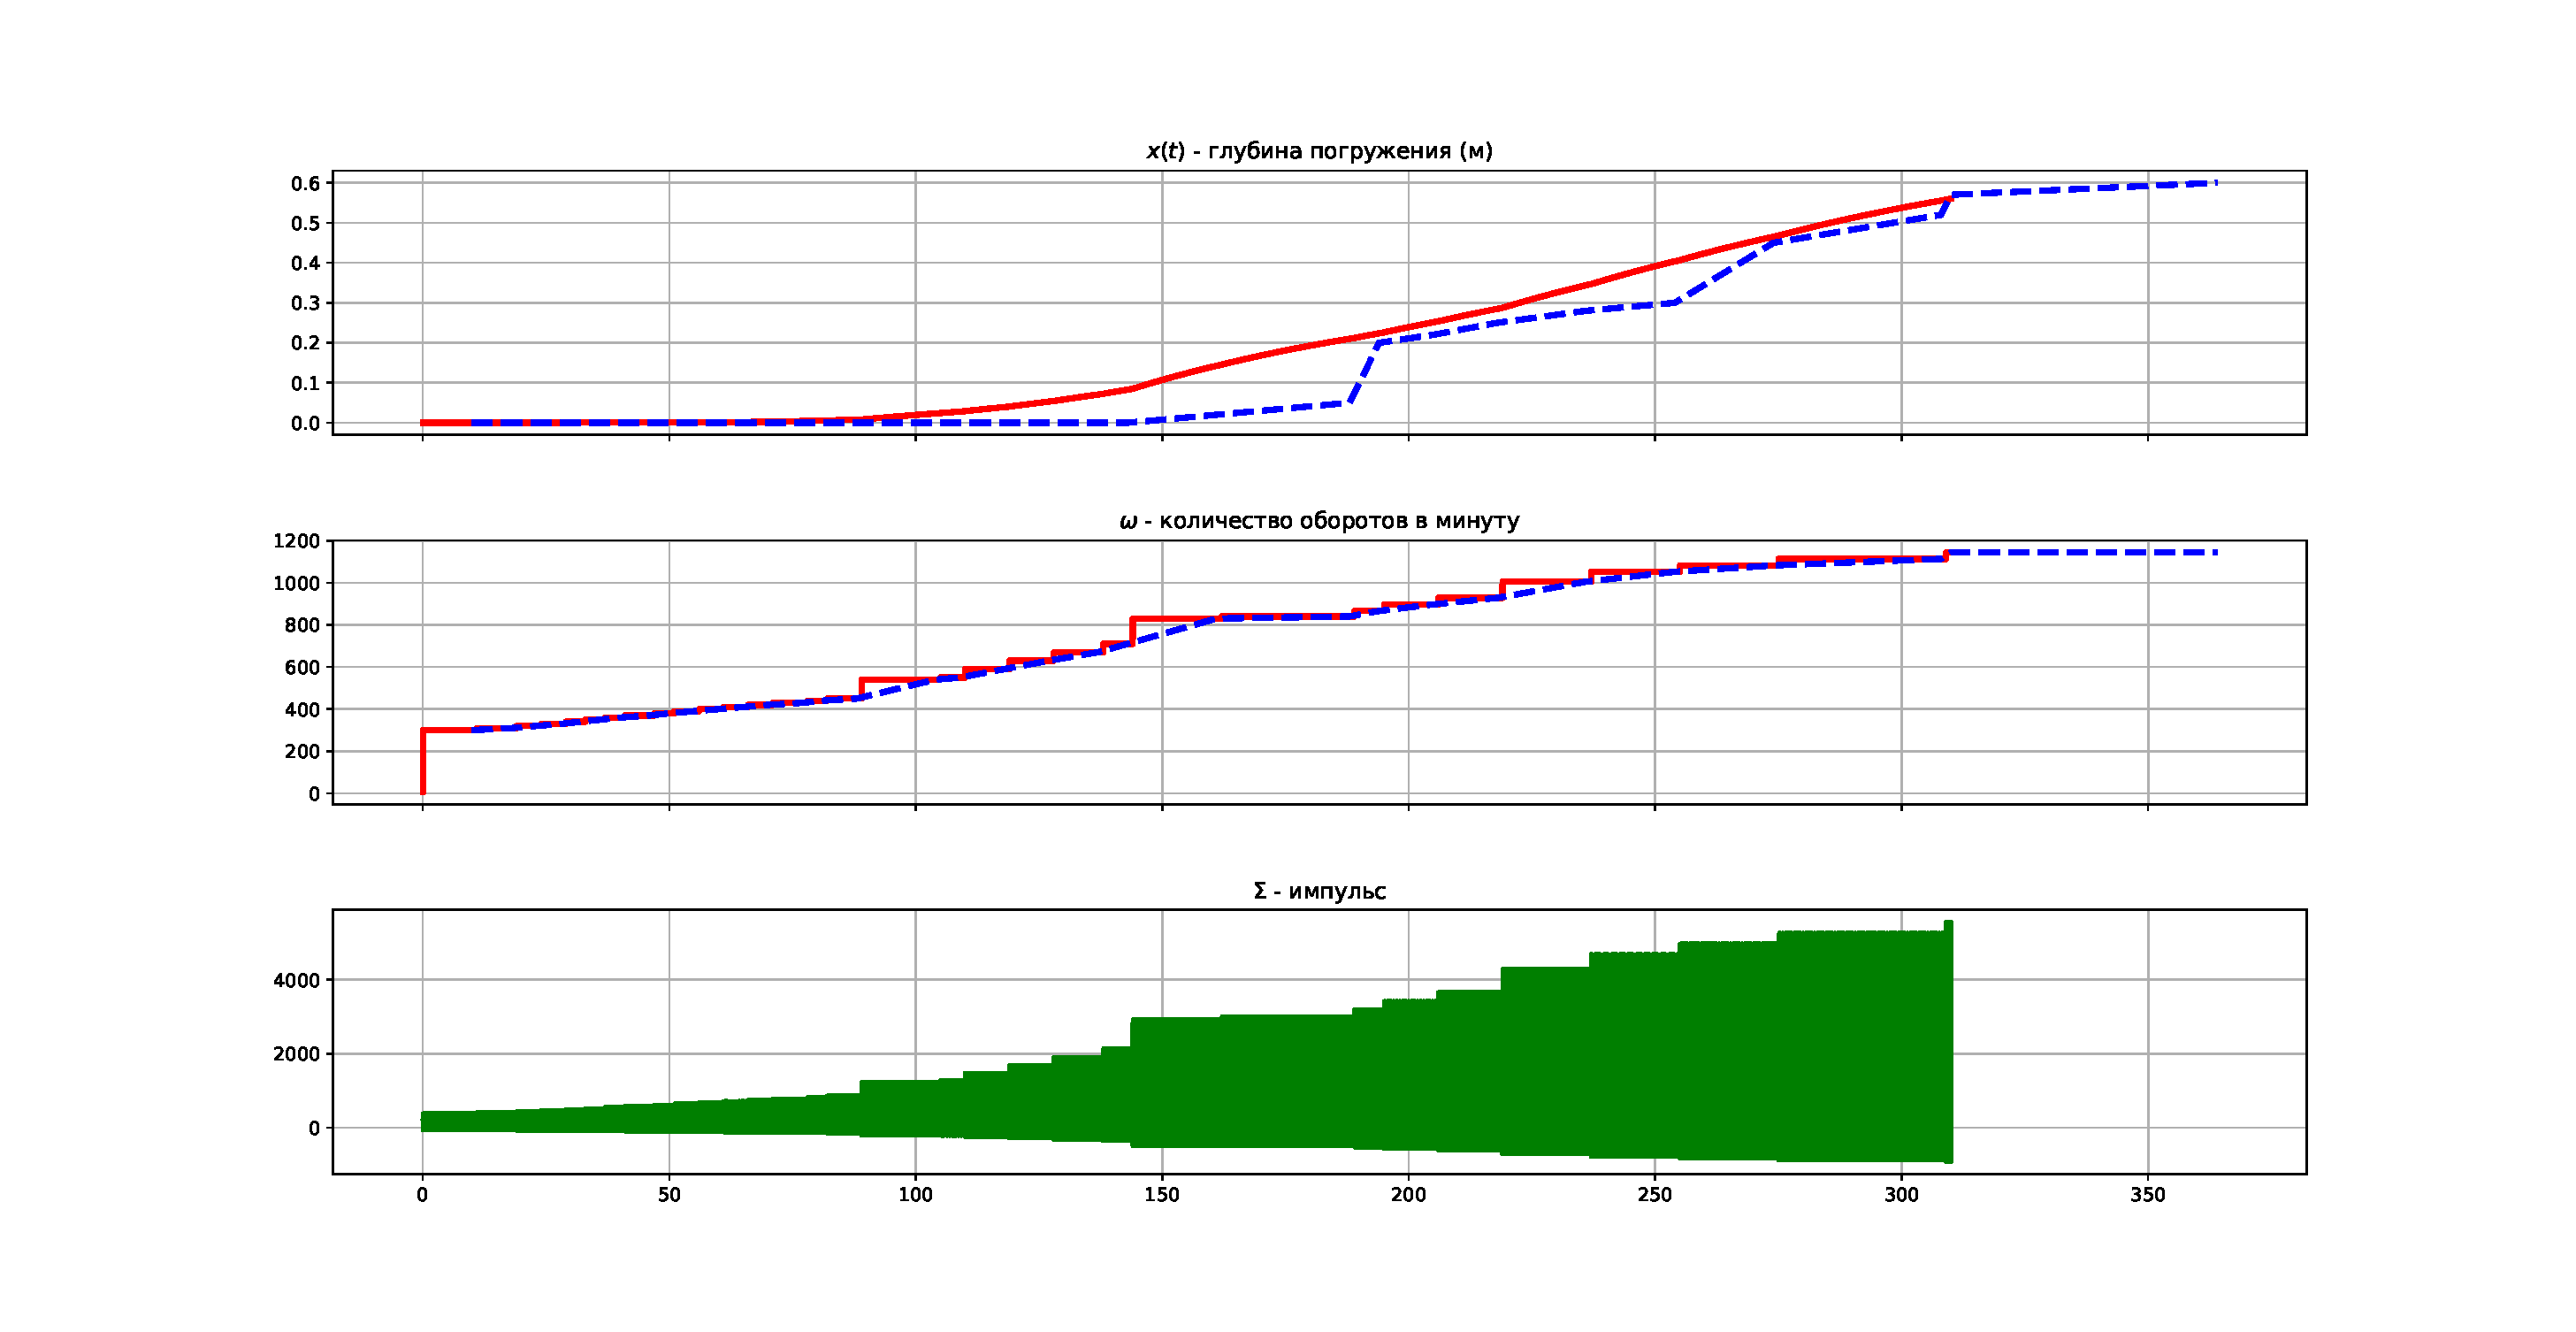
\includegraphics[width=1\linewidth]{graph}
            \caption{Сравнение результатов численного решения и результатов, полученных на практике.}
        \end{figure}
    \end{frame}

    \begin{frame}
        \begin{alertblock}{}
            \centerline{\color{darkred}Спасибо за внимание!}
        \end{alertblock}
    \end{frame}

\end{document}